\documentclass[12pt]{article}
\usepackage[spanish,es-nodecimaldot]{babel}
\usepackage[utf8]{inputenc}
\usepackage[T1]{fontenc}
\usepackage{newtxtext,newtxmath}
\usepackage[letterpaper,margin=1in]{geometry}
\usepackage{setspace}
\usepackage{graphicx}
\usepackage{booktabs}
\usepackage{array}
\usepackage{float}
\usepackage{url}
\usepackage{xurl}
\usepackage[hidelinks]{hyperref}
\usepackage{fancyhdr}
\usepackage{enumitem}
\usepackage{caption}
\usepackage{hanging}
\usepackage{tikz}
\usetikzlibrary{positioning,arrows.meta,shapes.geometric}
\setstretch{2}
\setlength{\parindent}{0.5in}
\setlength{\parskip}{0pt}
\setlength{\headheight}{15pt}
\pagestyle{fancy}
\fancyhf{}
\fancyhead[R]{\thepage}
\renewcommand{\headrulewidth}{0pt}
\captionsetup{font=small,labelfont=bf,labelsep=period}
\newcommand{\student}{Carlos Mario Salvatore Ocampo Aguilar}
\newcommand{\repo}{\href{https://github.com/Salv4tore27/carlos-transformers-series-tiempo-73437}{el repositorio público de GitHub}}
\newcommand{\colab}{\href{https://colab.research.google.com/github/Salv4tore27/carlos-transformers-series-tiempo-73437/blob/main/Carlos_Transformers_Series_Tiempo.ipynb}{cuaderno en Google Colab}}

\begin{document}
\begin{titlepage}
\thispagestyle{empty}
\centering
\vspace*{1.35in}
{\bfseries Atención temporal y Transformer para pronóstico de series de tiempo\par}
\vspace{1.2in}
\student\par
Universidad de Cundinamarca\par
Especialización en Inteligencia Artificial\par
Deep Learning -- Conceptos\par
R2-A3-S12 Transformers\par
Nidia Stella García Roa\par
19 de noviembre de 2026\par
\vfill
\end{titlepage}
\setcounter{page}{2}

\begin{center}
\textbf{Atención temporal y Transformer para pronóstico de series de tiempo}
\end{center}

\section{Introducción}
Una serie temporal no es una lista cualquiera de números: el orden de las observaciones contiene información. Si un modelo usa una ventana de valores recientes para estimar el siguiente, debe aprender qué partes de esa ventana ayudan más y conservar la secuencia temporal al entrenar y evaluar. Esta práctica aborda ese problema con dos mecanismos relacionados: atención temporal aditiva y un Transformer causal de tamaño reducido.

La arquitectura Transformer se propuso para procesar secuencias mediante atención, sin depender de recurrencia en cada paso (Vaswani et al., 2017). En pronóstico temporal, las variantes de atención pueden modelar relaciones a distintas escalas, aunque la arquitectura debe adaptarse al tamaño del conjunto y al horizonte requerido (Lim et al., 2021). Aquí se implementa un ejercicio de pronóstico de un paso que permite inspeccionar tanto el desempeño como los pesos de atención.

\section{Objetivos}
El objetivo general es comparar una atención aditiva sobre una ventana histórica con un Transformer causal básico, usando TensorFlow y Keras para predecir el valor siguiente de una serie temporal. En concreto, se prepara una señal con componentes conocidos, se separa cronológicamente en entrenamiento y prueba, se entrenan ambos modelos con validación temporal y se comparan con una predicción de persistencia mediante MAE y RMSE.

\section{Fundamento técnico}
\subsection{Atención}
La atención asigna pesos a representaciones de una secuencia. En la formulación escalada de producto punto, se combinan consultas, claves y valores mediante
\begin{equation}
\operatorname{Attention}(Q,K,V)=\operatorname{softmax}\left(\frac{QK^{\mathsf T}}{\sqrt{d_k}}\right)V.
\end{equation}
La operación convierte las puntuaciones en una distribución de pesos y produce un contexto ponderado. La atención aditiva de esta práctica calcula una puntuación para cada posición a partir de la representación de esa observación y de una consulta asociada al extremo reciente de la ventana; luego agrega los valores con esos pesos. La idea de aprender qué fragmentos de una secuencia importan se relaciona con los mecanismos de alineación neuronal de Bahdanau et al. (2015).

\subsection{Transformer temporal}
El modelo transforma cada observación escalar en un vector de 32 componentes, suma una codificación posicional aprendible y aplica una capa de autoatención multi-cabeza con cuatro cabezas. Una máscara causal impide que una posición atienda a posiciones posteriores dentro de la secuencia. La salida de atención se combina con la entrada mediante conexión residual y normalización; una red densa de tipo feed-forward refina cada representación. Para el pronóstico de un paso se usa la representación del último instante de la ventana.

La codificación posicional es necesaria porque la autoatención, por sí sola, no conserva el orden de los datos. La lectura asignada presenta el flujo de entradas, posiciones, atención y máscara como una secuencia de transformaciones; en este ejercicio, esas mismas ideas se trasladan de tokens a instantes de una señal numérica (Doshi, 2021). Aunque un Transformer puede procesar en paralelo todas las posiciones de entrada, el pronóstico exige respetar el tiempo: los datos futuros no deben participar en el ajuste ni en el cálculo del contexto. Por eso, el corte y la máscara causal forman parte del diseño, no son solo detalles de implementación.

\section{Método}
\subsection{Serie y preparación}
Se generó una serie sintética de 720 puntos con una tendencia lineal suave, oscilaciones de período 24, 8 y 72 pasos, y ruido gaussiano. La señal representa únicamente un índice de demanda didáctico; no son datos medidos ni se atribuye a una organización o servicio real. Esta decisión permite repetir el experimento sin descargar datos externos, pero limita las conclusiones a la señal construida.

Se reservó el primer 80\% de los puntos para entrenamiento y el último 20\% para prueba. La normalización se ajustó solamente con el tramo previo al corte. Cada ejemplo contiene los 36 valores anteriores y tiene como objetivo el punto inmediatamente siguiente. Dentro del tramo de entrenamiento, el 15\% más reciente se separó para validación. En la prueba se aplicó evaluación de un paso: a medida que avanza el tramo, las observaciones previas ya ocurridas pueden entrar en la ventana. Esta separación temporal evita mezclar aleatoriamente pasado y futuro (Hyndman \& Athanasopoulos, 2021).

\subsection{Modelos y entrenamiento}
El script \texttt{experimento\_transformers.py} contiene cuatro bloques: generación de serie y ventanas; construcción de los modelos; entrenamiento con detención temprana según la pérdida de validación; y cálculo de métricas y figuras. El modelo de atención aditiva proyecta la ventana a 32 dimensiones y obtiene un contexto ponderado. El Transformer utiliza codificación posicional, autoatención causal, normalización y red feed-forward. Ambos se optimizan con Adam y error cuadrático medio, hasta 35 épocas, con tamaño de lote 32 y paciencia 5 para detenerse si la validación no mejora.

Se repitió el ajuste con tres semillas (13, 27 y 41) para observar sensibilidad a la inicialización. Como referencia simple se incluyó persistencia: pronosticar que el siguiente valor será igual al último de la ventana. Las métricas se calcularon en la escala original de la señal. MAE resume el error absoluto promedio; RMSE penaliza con más fuerza los errores grandes. No se usa MAPE porque la serie puede tomar valores cercanos a cero.

\begin{figure}[H]
\centering
\begin{tikzpicture}[
  node distance=0.48cm and 0.58cm,
  box/.style={draw=black!55, rounded corners=2pt, align=center, minimum height=0.82cm, text width=2.15cm, fill=blue!6, font=\small},
  model/.style={box, fill=orange!12, text width=2.15cm},
  arrow/.style={-{Latex[length=2mm]}, thick, draw=black!65}
]
\node[box] (serie) {\shortstack{Serie sintética\\720 puntos}};
\node[box, right=of serie] (ventana) {\shortstack{Ventanas\\de 36 pasos}};
\node[box, right=of ventana] (split) {\shortstack{Corte temporal\\80\% / 20\%}};
\node[model, right=1.0cm of split, yshift=0.65cm] (att) {\shortstack{Atención\\aditiva}};
\node[model, right=1.0cm of split, yshift=-0.65cm] (trans) {\shortstack{Transformer\\causal}};
\node[box, right=1.0cm of att, yshift=-0.65cm, fill=green!10] (eval) {\shortstack{MAE, RMSE\\y persistencia}};
\draw[arrow] (serie) -- (ventana);
\draw[arrow] (ventana) -- (split);
\draw[arrow] (split.east) -- ++(0.35,0) |- (att.west);
\draw[arrow] (split.east) -- ++(0.35,0) |- (trans.west);
\draw[arrow] (att.east) -- (eval.west);
\draw[arrow] (trans.east) -- (eval.west);
\end{tikzpicture}
\caption{Flujo de preparación, modelado y evaluación del experimento.}
\end{figure}

\begin{figure}[H]
\centering
\IfFileExists{resultados/serie_particion.png}{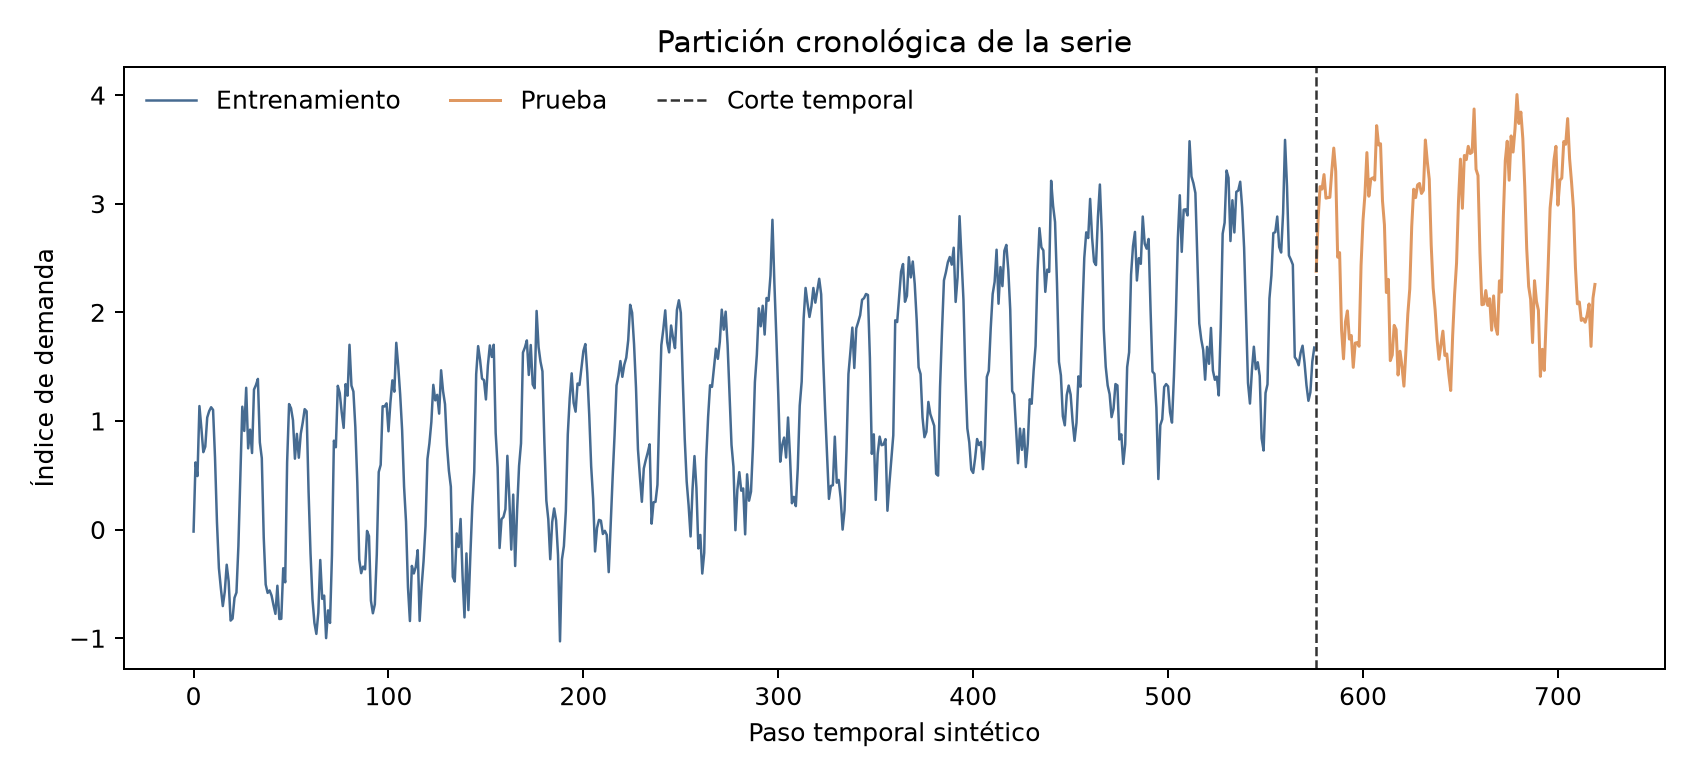
\includegraphics[width=0.88\linewidth]{resultados/serie_particion.png}}{\fbox{Ejecutar el notebook para generar la figura de partición temporal.}}
\caption{Serie sintética y separación cronológica de entrenamiento y prueba.}
\end{figure}

\section{Resultados}
La ejecución en Colab se realizó con TensorFlow 2.21.0. La tabla presenta el resultado de persistencia y el promedio y desviación estándar de las tres semillas para cada modelo entrenable. Las métricas se reportan en la escala original de la señal sintética.

\begin{table}[H]
\centering
\caption{Error en el conjunto de prueba}
\begin{tabular}{lcc}
\toprule
Modelo & MAE & RMSE \\
\midrule
Persistencia & 0.270 & 0.335 \\
Atención aditiva (media $\pm$ DE) & 0.722 $\pm$ 0.002 & 0.800 $\pm$ 0.005 \\
Transformer (media $\pm$ DE) & 0.424 $\pm$ 0.032 & 0.510 $\pm$ 0.048 \\
\bottomrule
\end{tabular}
\vspace{0.18in}
\begin{minipage}{0.88\linewidth}\small\textit{Nota.} DE = desviación estándar entre las semillas 13, 27 y 41. Menor valor indica menor error.\end{minipage}
\end{table}

\begin{figure}[H]
\centering
\IfFileExists{resultados/comparacion_rmse.png}{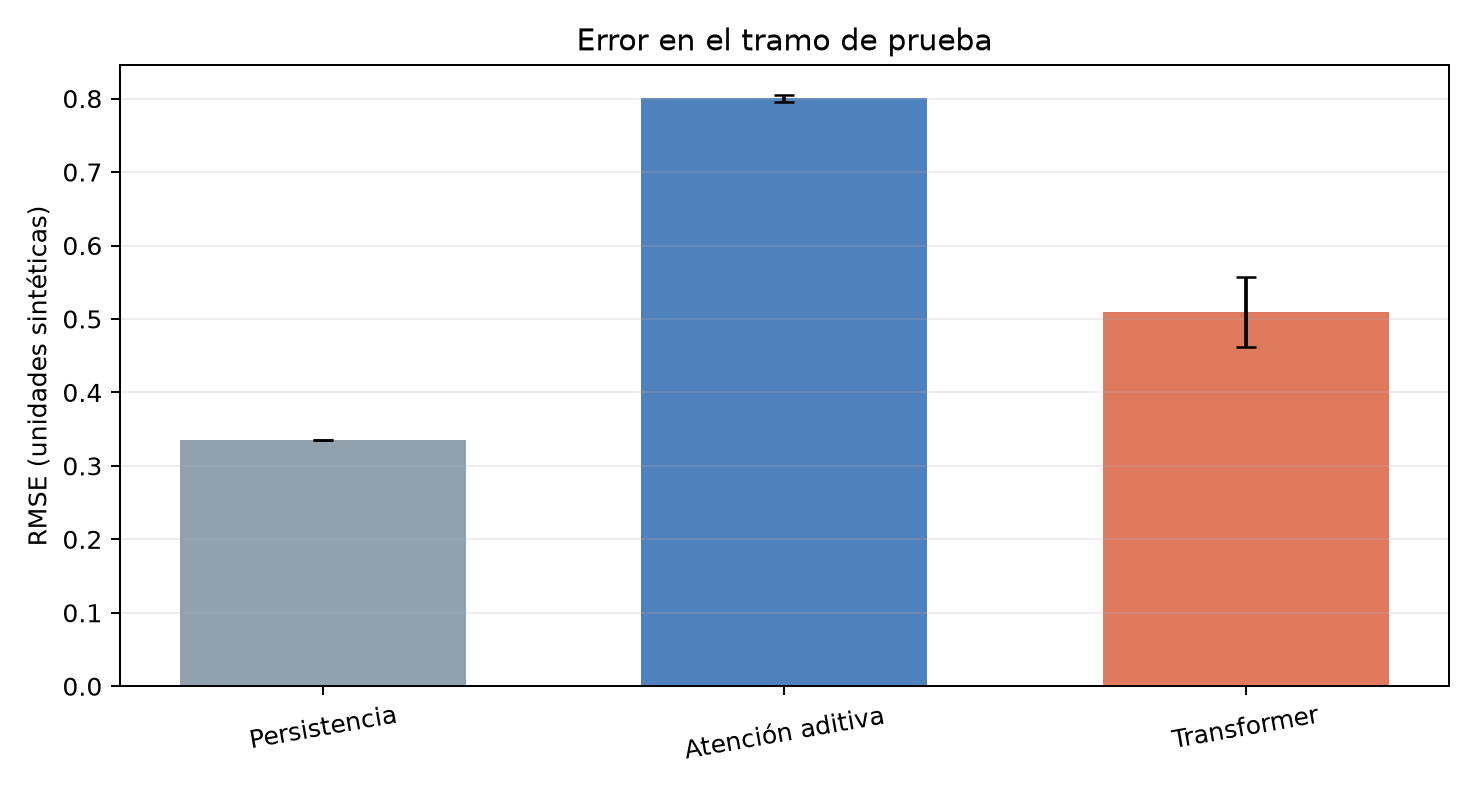
\includegraphics[width=0.78\linewidth]{resultados/comparacion_rmse.png}}{\fbox{Ejecutar el notebook para generar la comparación de RMSE.}}
\caption{Comparación de RMSE entre persistencia, atención aditiva y Transformer.}
\end{figure}

El cuaderno incluye además la visualización de los pesos asignados por la atención aditiva a una ventana de prueba. Esos pesos permiten revisar cómo se distribuye la ponderación entre instantes; no deben interpretarse como evidencia causal.

\subsection{Interpretación}
La persistencia obtuvo el menor error (MAE = 0.270; RMSE = 0.335). El Transformer redujo el error frente a la atención aditiva, pero no superó la referencia simple: su MAE fue 0.424 y su RMSE 0.510. La atención aditiva presentó los errores más altos (MAE = 0.722; RMSE = 0.800). En esta señal, la autocorrelación de corto plazo hace que copiar el último valor sea una estrategia difícil de superar; por eso el resultado no favorece automáticamente a los modelos más complejos.

La dispersión entre semillas fue menor para la atención aditiva que para el Transformer. Sin embargo, esa estabilidad no compensa su error promedio más alto. El gráfico de pesos permite inspeccionar qué posiciones recibió más importancia el mecanismo aditivo; esos pesos describen la operación del modelo, pero no constituyen por sí solos una explicación causal.

\section{Discusión}
La práctica materializa los elementos indicados en la consigna: embeddings numéricos de observaciones, codificación posicional, self-attention, máscara causal, entrenamiento y evaluación en secuencias. La atención aditiva sirve como mecanismo explícito y compacto de ponderación; el Transformer agrega autoatención multi-cabeza y transformaciones por posición. La implementación es intencionalmente pequeña para que cada componente pueda revisarse en el cuaderno.

La comparación tiene limitaciones importantes. La serie es artificial, univariada y regular; no contiene cambios de régimen, estacionalidad cambiante ni covariables. La tarea es un paso adelante y no mide desempeño a horizontes largos. Además, se usa una sola partición final y tres inicializaciones, no validación de origen rodante. Por eso, no corresponde extrapolar los errores a demanda real ni afirmar superioridad general del Transformer. Un siguiente experimento debería usar una serie pública documentada, más horizontes y ventanas de evaluación rodante.

\section{Conclusiones}
Se implementaron dos formas de atención para el análisis de una serie temporal: una ponderación aditiva de los instantes de la ventana y una arquitectura Transformer causal con codificación posicional. La evaluación cronológica y la normalización ajustada solo en entrenamiento mantienen la comparación separada del futuro. La persistencia ofrece un punto de referencia necesario para decidir si el aprendizaje agrega valor.

En esta ejecución, la persistencia fue el mejor método y el Transformer superó a la atención aditiva, aunque ambos quedaron por debajo de la referencia. La conclusión se apoya en métricas del tramo de prueba y tres semillas, no en la complejidad teórica de cada arquitectura. Los resultados describen únicamente la señal sintética. Para trasladar el método a una aplicación real se requiere una fuente de datos con procedencia, más de un horizonte, análisis de errores por período y validación temporal repetida.

\section*{Código y evidencias}
El notebook ejecutado está disponible en \colab. El código fuente, el informe y los resultados se organizan en \repo. El notebook genera \texttt{resumen.json}, \texttt{metricas\_semillas.csv}, \texttt{predicciones\_prueba.csv} y las figuras de evidencia. El informe debe compilarse junto con la carpeta \texttt{resultados/}.

\section*{Referencias}
\begin{hangparas}{0.5in}{1}
Bahdanau, D., Cho, K., \& Bengio, Y. (2015). Neural machine translation by jointly learning to align and translate. En \textit{3rd International Conference on Learning Representations}. \url{https://arxiv.org/abs/1409.0473}

Doshi, K. (2021, January 2). Transformers explained visually (Part 2): How it works, step-by-step. \textit{Towards Data Science}. \url{https://towardsdatascience.com/transformers-explained-visually-part-2-how-it-works-step-by-step-b49fa4a64f34/}

Hyndman, R. J., \& Athanasopoulos, G. (2021). \textit{Forecasting: Principles and Practice} (3rd ed.). OTexts. \url{https://otexts.com/fpp3/}

Lim, B., Arık, S. Ö., Loeff, N., \& Pfister, T. (2021). Temporal fusion transformers for interpretable multi-horizon time series forecasting. \textit{International Journal of Forecasting, 37}(4), 1748--1764. \url{https://doi.org/10.1016/j.ijforecast.2021.03.012}

Vaswani, A., Shazeer, N., Parmar, N., Uszkoreit, J., Jones, L., Gomez, A. N., Kaiser, Ł., \& Polosukhin, I. (2017). Attention is all you need. En \textit{Advances in Neural Information Processing Systems} (Vol. 30). \url{https://arxiv.org/abs/1706.03762}
\end{hangparas}

\end{document}
